\documentclass[a4paper,12pt]{article}
\usepackage[left=2.5cm,right=2.5cm,top=2.5cm,bottom=2.5cm]{geometry} 
\usepackage{amsmath,amssymb,amsthm,algorithm,algorithmic,graphicx,yhmath,url,enumitem,lscape,hyperref}
\usepackage{wrapfig,subfigure}
\usepackage{lineno}

\newcounter{problem}
\newcounter{remark}
\newcounter{hint}
\newenvironment{remark}{\refstepcounter{remark} \vspace{0.1cm} \par \noindent {\bf Remark \arabic{remark}}}{\vspace{0.3cm}}
\newenvironment{hint}{\refstepcounter{hint} \vspace{0.1cm} \par \noindent {\bf Hint \arabic{hint}}}{\vspace{0.3cm}}
\newcommand{\R}{\mathbb{R}}
\newcommand{\N}{\mathbb{N}}
\newcommand{\Rn}{\mathbb{R}^n}
\newcommand{\Rnn}{\mathbb{R}^{n \times n}}
\newcommand{\bes}{\begin{equation*}}
\newcommand{\ees}{\end{equation*}}
\newcommand{\be}{\begin{equation}}
\newcommand{\ee}{\end{equation}}
\newcommand{\bms}{\begin{multline*}}
\newcommand{\emults}{\end{multline*}}

% Matrices
\newcommand{\bbm}{\begin{bmatrix}}
\newcommand{\ebm}{\end{bmatrix}}
\newcommand{\bpm}{\begin{pmatrix}}
\newcommand{\epm}{\end{pmatrix}}

% Strecthing
\renewcommand{\arraystretch}{1.3}

\newcommand{\eps}{\epsilon}
\newcommand{\fl}{\text{fl}}
\newcommand{\Lp}{{L^p}}
\newcommand{\Ker}{\text{Ker}\,}
\newcommand{\loc}{{\text{loc}}}
\newcommand{\ccinf}{C_c^\infty}
\newcommand{\supp}{\text{supp}}
\newcommand{\dist}{\text{dist}}

% Gravitational acceleration
\newcommand{\bg}{\mathbf{g}}
% Friction force
\newcommand{\bFf}{\mathbf{F_f}}
% Gravitational force
\newcommand{\bFg}{\mathbf{F_g}}
% Force
\newcommand{\bF}{\mathbf{F}}
% Position, velocity, acceleration
\newcommand{\br}{\mathbf{r}}
\newcommand{\bv}{\mathbf{v}}
\newcommand{\ba}{\mathbf{a}}

% Jacobian
\newcommand{\bDF}{\mathbf{DF}}

\newtheorem{theorem}{Theorem}[section]
\newtheorem{proposition}[theorem]{Proposition}
\newtheorem{lemma}[theorem]{Lemma}
\newtheorem{definition}[theorem]{Definition}
\title{Robust and accurate root finding for real polynomials}
\author{Carl Christian Kjelgaard Mikkelsen}

\begin{document} 

\pagenumbering{arabic}
% Turn off line numbering by commenting the following line.
\linenumbers
\thispagestyle{empty}

\noindent
Ume\aa{} University \hfill Fall 2018 \\
Department of Computing Science\\

\vskip 2.5cm

\begin{center} {\Huge {\bf Project 1}}\\{\Large Robust and accurate root finding for real polynomials}\end{center} \vskip 0.3cm
\begin{center}
  {\huge Scientific Computing}
  \vfill
  {\Large The deadline for this project can be found at: \href{http://www8.cs.umu.se/kurser/5DV005/HT18/planering.html}{http://www8.cs.umu.se/kurser/5DV005/HT18/planering.html}\\
  (Link \emph{Overview} on the course homepage.)}
\end{center}
  \vfill
  {% \large
\begin{itemize}
\item The submission should consist of:
  \begin{itemize}
  \item The complete report, including
    \begin{itemize}
    \item A front page with the following information:
      \begin{enumerate}
      \item Your {\bf name}.
      \item The {\bf course name}.
      \item Your {\bf username} at the Department of Computing
        Science.
      \item The {\bf project number}.
      \item The {\bf version} of the submission (in case of re-submissions).
      \end{enumerate}
    \end{itemize}
  \item An appendix with the source code.
  \item To simplify feedback, the main report (optionally excluding
    the appendix) must have {\bf numbered sections} and {\bf page
      numbers}.
  \end{itemize}
\item The submitted code must be Matlab-compatible. If you choose to
  work in Octave, verify that your code is Matlab-compatible before
  you submit your project.
\item If you write your report using \LaTeX, double-check that your
  references have been resolved correctly before you submit. ``Figure ??'' is useless to any reader.
\item Your report should be submitted as a pdf file uploaded via
  the\linebreak 
  \href{https://webapps.cs.umu.se/labresults/v2/handin.php?courseid=337}{https://webapps.cs.umu.se/labresults/v2/handin.php?courseid=337}
  page, also available as the
\begin{center}
  \href{http://www8.cs.umu.se/kurser/5DV005/HT18/index2.html}{Submit/Check results}
\end{center} link at the bottom left of the course home page.
\item Furthermore, every scrap of MATLAB code developed by your team should be uploaded in a single zip file, {\tt P1Code.zip}.
\end{itemize}
  }
  \vfill

\newpage



\maketitle

\tableofcontents
\listoffigures

\section{What makes a good report?}

A good report has lasting value for end user as well as the author. A good reports can be read without referring to the assignment specification. A good report has a clear structure. It has a meaningful title, a list of contributors, a table of contents, a list of figures and a list of tables both with short meaningful titles. An introduction describes the overall purpose of the report and lists the topics that will be discussed. Subsequent sections are dedicated to individual topics. Relevant questions are clearly formulated and answered. The writer's reasoning is explained and all claims are carefully supported. Tables and pictures with meaningful labels and captions are presented and relevant details are discussed. Appropriate references are made to other reports, books, or appendices. A good report ends with a summary of the results obtained, a list of any unresolved issues and suggestions for future work.

\section{Purpose} In this project you will develop a function {\tt my\_root} which can be used to compute all real roots of a real polynomial $y = p(x)$ on the real line.
The function will automatically detect and abort if the sign of the computed value $\hat{y}$ can not be trusted. When developing software your priorities are robustness, accuracy and speed in that order. This project will demonstrate how to write numerical software which is aware of its own limitations and can issue appropriate warnings.

\section{Motivation}

Polynomials and rational functions are the only functions we can compute using the basic arithmetic operations. Fortunately, all other functions can be approximated using these operations. In the world of computational science there are two kinds of problems:
\begin{itemize}
\item computing function values, and
\item solving equations.
\end{itemize}
If we can not accomplish these task for polynomials in a manner which is robust, accurate and fast, then we should not attempt to solve more complicated problems.

\section{Construction of test cases} 

When developing software one must also develop test cases which can be used to detect bugs. The test cases must be so complex that all branches of the code are executed. For numerical software, the examples must be chosen such that we know the correct result. Frequently, it is practical to compute all intermediate results by hand or using another program. Well chosen test cases can reveal bugs, but only careful analysis of the program can eliminate bugs.

In the context of root finding for polynomials, we require polynomials which are simple to define and have known roots which can be computed accurately. One such class of polynomials are the Chebyshev polynomials $T_n$ of the first kind. They are given by the following linear recurrence relation
\begin{align}
  T_0(x) &= 1 \\
  T_1(x) &= x \\
  T_{j+1} &= 2x T_j(x) - T_{j-1}(x), \quad j \in \{1,2,3,\dotsc\}.
\end{align}

\begin{enumerate}
\item Find the explicit formula for $T_n$ for $n=3,4,5,6$ by hand.
\item Show by induction that $T_n$ has degree $n$. Consult the examples given in Chapter 3 of \cite{mikkelsen2018} to see how proofs by induction are written properly.
\item Copy {\tt no1/scripts/a1f1.m} into {\tt no1/work/MyChebyshev.m} and complete the function according to the specifications. The function must compute $T_j(x)$ for $j=0,1,2,\dots,n-1$ and $x \in X$, where $X$ is an arbitrary array.
\item Copy {\tt no1/scripts/a1f2.m} into {\tt no1/work/MyChebyshevMWE1} and complete the script so that it generates a figure similar to Fig \ref{fig:PlotChebyshev}.
\end{enumerate}

\begin{figure}
  \centering
  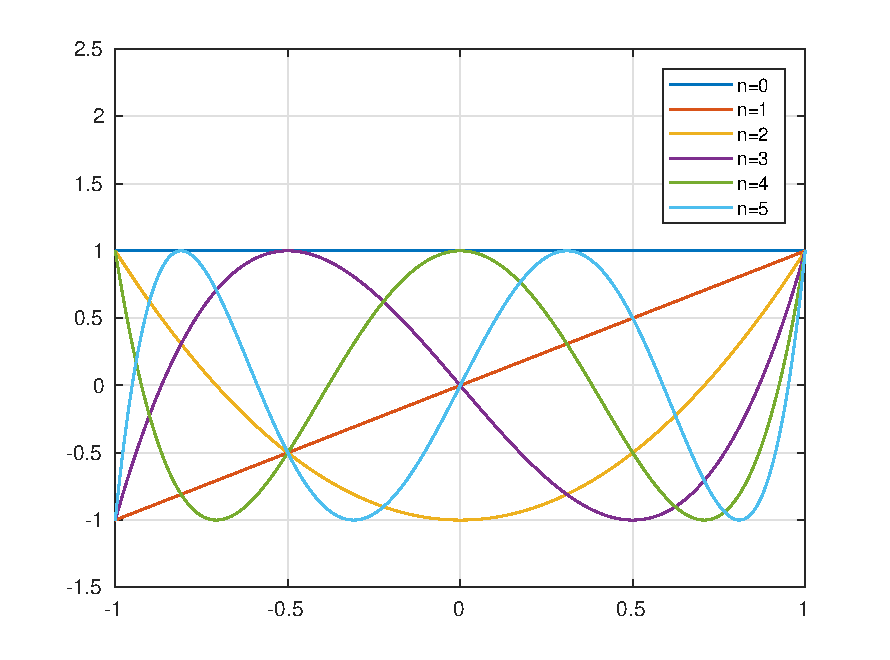
\includegraphics[width=0.7\textwidth]{PlotChebyshev.pdf} \caption[Plot of the first few Chebyshev polynomials of the first kind.]{A plot of the first $n=6$ Chebyshev polynomials of the first kind.} \label{fig:PlotChebyshev}
\end{figure}


It is straightforward, but tedious to verify that, say, $T_{10}$ is given by
\be
T_{10}(x) = 512 x^{10} - 1280 x^8 + 1120 x^6 - 400 x^4 + 50 x^2 - 1,
\ee
but it is not at all obvious what the roots might be!

The following theorem can be used without proof.

\begin{theorem} The Chebyshev polynomials of the first kind satisfy the equation
  \be
T_n(\cos(\theta)) = \cos(n\theta), \quad \theta \in \R.
\ee
\end{theorem}

\begin{enumerate}[resume]
\item Show that the $n$ roots of $T_n$ are given by
  \be \label{equ:exact-roots}
  x_k = \cos\left(\frac{(2k-1)\pi}{2n}\right), \quad k = 1,2,\dots,n.
  \ee
\end{enumerate}

\begin{hint} If you do not exploit the fact that $T_n$ has degree $n$ and if you do not reference the Fundamental Theorem of Algebra, then your proof is not complete.
\end{hint}

\begin{remark} It is worth observing that the coefficients of $T_n$ are all integers. These integers are small enough to be exactly representable in, say, double precision floating point arithmetic, at least for small values of $n$. The roots of $T_n$ are contained in the interval $[-1,1]$, hence we know where our solver should look. Moreover, the roots can be computed accurately from formula \eqref{equ:exact-roots} except near the middle of the interval as $x \to \cos(x)$ is ill conditioned near $x = \frac{\pi}{2}$. These properties all excellent qualities for a test case.
\end{remark}

\section{Root finding software}

If $f : \mathbb{R} \rightarrow \mathbb{R}$ is continuous and $f(a)$ and $f(b)$ have different sign, then there exists a zero of $f$ between $a$ and $b$. We say that $a$ and $b$ bracket the root. In floating point we cannot necessarily trust the computed value of the sign of $y = f(x)$. If $f$ is a polynomial, then we can compute a running error bound, i.e., a number $\mu$ such that
\be
|y - \hat{y}| \leq \mu u
\ee
where $\hat{y}$ is the computed value of $y = f(x)$ and $u$ is the unit roundoff. If $|\hat{y}| > \mu u$, then $y$ and $\hat{y}$ have the same sign, i.e., the computed value of the sign of $y$ is correct. If $|\hat{y}| \leq \mu u$, then $y$ and $\hat{y}$ need not have the same sign. In particular, $y=0$ is a distinct possibility and $x$ could be a root.

\begin{enumerate}
\item Copy {\tt no1/scripts/a1f3.m} into {\tt no1/work/MyRoot.m} and complete the function according to its specification. In particular, {\tt MyRoot} must evaluate your polynomial $y=p(x)$ and error bounds using your function {\tt my\_horner} and it must use the bisection algorithm to refine a bracket around a root. {\tt MyRoot} must reject the initial bracket if the computed sign of $p(a)$ and $p(b)$ cannot be trusted or if the computed signs can be trusted and are identical. The function must terminate and return $x$ if the computed sign of $y=p(x)$ cannot be trusted.
\item Develop a minimal working example {\tt no1/work/MyRootMWE1} which finds good approximations of all roots of $T_{10}$ and displays all information in a nice table. The results for $T_6$ should be similar to Figure \ref{fig:MyRootMWE6}.

  \begin{hint} The class repository contains an auxiliary function {\tt displaytable} which can be used to print tables nicely. It is worth your time to learn who to use this function, see {\tt compute\_range} for an illustration.
\end{hint}

\begin{landscape}
\begin{figure}
  \begin{verbatim}
 Idx | flag | iter |              a |            b |         root |     residual |          REB | trust
   1 |    1 |   29 |    -9.6593e-01 |  -9.6593e-01 |  -9.6593e-01 |  -7.2711e-10 |   1.6115e-14 |     1
   2 |    2 |   26 |    -7.0711e-01 |  -7.0711e-01 |  -7.0711e-01 |   3.0926e-11 |   5.3291e-15 |     1
   3 |    2 |   26 |    -2.5882e-01 |  -2.5882e-01 |  -2.5882e-01 |   5.6922e-11 |   5.3867e-16 |     1
   4 |    2 |   26 |     2.5882e-01 |   2.5882e-01 |   2.5882e-01 |   5.6922e-11 |   5.3867e-16 |     1
   5 |    2 |   26 |     7.0711e-01 |   7.0711e-01 |   7.0711e-01 |   3.0926e-11 |   5.3291e-15 |     1
   6 |    1 |   29 |     9.6593e-01 |   9.6593e-01 |   9.6593e-01 |  -7.2711e-10 |   1.6115e-14 |     1
\end{verbatim} \caption[Root finding for $T_6$.]{The result of applying {\tt MyRoot} to the polynomial $T_6$. Initially, $m=101$ equidistant points in the interval $[-1,1]$ where used to define (potential) brackets. Tolerance {\tt delta = 1e-10} and {\tt eps=1e-10} were used to control the bisection process. Notice the variation in the flags and iteration counts returned by {\tt MyRoot} and the fact that the sign checks are positive.} \label{fig:MyRootMWE6}
  \end{figure}
\end{landscape}



\end{enumerate}

\section{Calculations}

\begin{enumerate}
\item Find all $n$ roots of $T_n$ for $n=10$ with a relative error less than $\tau = 10^{-13}$ using {\tt MyRoot}.
\item For each root explain, why your calculations can be trusted.
  \begin{hint}
    If your explanation does not refer to relevant brackets and running error bounds, then it not complete.
  \end{hint}
\end{enumerate}

\begin{remark}
  The vast majority of users are completely ignorant of floating point arithmetic and will blindly rely on the results produced by a computer program.  Sadly, many codes are written by intelligent people who are blissfully unaware of the limitations of floating point arithmetic. It is our responsibility to write code which is reliable, sufficiently accurate for the task at hand, and sufficiently fast.
\end{remark}

 \bibliographystyle{plain}
  \bibliography{../../../lecture-notes/refs}

\end{document}

